% Original proposed method. This manuscript contains no measured benchmark results.
\documentclass{article}
\usepackage{iclr2027_conference,times}
\usepackage[T1]{fontenc}
\usepackage{amsmath,amssymb,booktabs,tabularx,graphicx,hyperref,url}
\usepackage{tikz,etoolbox}
\usetikzlibrary{arrows.meta,positioning,fit,backgrounds}
\hypersetup{colorlinks=true,linkcolor=blue,citecolor=blue,urlcolor=blue}
\newcommand{\KB}{\mathcal{K}}
\newcommand{\EB}{\mathcal{E}}
\newcommand{\WM}{w}
\newcommand{\Model}{\pi_{\theta}}
\title{Learning to Remember from Failure:\\Knowledge, Experience, and Working Memory}
\author{Anonymous authors}
% Working-copy labels; the official conference style remains unmodified.
\makeatletter
\patchcmd{\@maketitle}{Paper under double-blind review}{Manuscript in preparation}{}{}
\makeatother

\begin{document}
\maketitle
\lhead{Working manuscript: empirical evaluation pending}

\begin{abstract}
Conversational memory can fail because evidence was discarded, relevant records
were not retrieved, or retrieved evidence was used incorrectly. Repeating the
same memory pipeline does not distinguish these failures. We propose a framework
with two persistent banks and one transient working state: a knowledge bank
stores source-grounded facts, an experience bank stores reusable repair
procedures, and working memory tracks the evidence still needed for the current
question. Experience controls how knowledge is encoded, retrieved, and used;
only the knowledge bank can supply factual support for an answer. Failed
development trajectories produce candidate procedures, which are retained only
after controlled replay and validation. The model weights remain fixed.
We specify three focused experiments on LoCoMo and LongMemEval: answer quality
and cost, the contribution of the three memory roles, and transfer as experience
accumulates. This manuscript presents the method and experimental protocol;
benchmark results have not yet been measured.
\end{abstract}

\section{Introduction}
A memory-augmented agent may answer a question about a user's current residence
with an old address. Three different failures can produce that answer: the move
was omitted during memory construction, the new address was stored but not
retrieved, or both addresses were retrieved without comparing their dates.
These failures call for different interventions. An extra search cannot recover
information that was never retained, while a better writer cannot by itself
resolve a reader's temporal mistake.

Existing systems make complementary advances in memory extraction, organization,
and efficient retrieval \citep{mem0,amem,simplemem,lightmem}. Experience-based
agents reuse feedback and prior attempts \citep{reflexion,adamem,reme}.
Yet a conversational memory system still needs an explicit connection between
\emph{what it remembers} and \emph{what it has learned about remembering}.
We study that connection through three roles: persistent knowledge, persistent
experience, and transient working state.

The proposed mechanism is \emph{failure-directed memory repair}. A trace records
which facts were available, what was retrieved, and which evidence supported the
answer. A learner tests a small repair to the writer, retriever, or reader and
distills a successful intervention into a reusable conditional procedure.
Future questions retrieve these procedures as guidance, while their factual
answers remain grounded in the current conversation's knowledge bank. Working
memory connects the two banks by exposing missing evidence and failed attempts.

The memory taxonomy itself is established \citep{langmem}. Recuris already uses
working state to select experience and localizes failures for memory-control
updates \citep{recuris}. Our proposed distinction is the repair of a separate
\emph{factual} bank and its evidence-access pipeline for conversational QA. This
distinction is a hypothesis to test, rather than a claim of demonstrated
superiority. The contribution of this draft is a concrete architecture, a
bounded repair procedure, and an evaluation that separates factual recall from
cross-question procedural transfer.

\section{Three Memory Roles}
\label{sec:method}
Let $H_i$ be the timestamped dialogue history associated with question $q_i$.
The agent uses a frozen language model $\Model$ and memory
\begin{equation}
    M_{i,t}=(\KB_i,\EB_n,\WM_{i,t}),
\end{equation}
where $\KB_i$ is scoped to the history, $\EB_n$ contains experience accepted
after development stage $n$, and $\WM_{i,t}$ exists only during the current
question. Histories belonging to the same conversation may reuse their
knowledge bank; unrelated users or evaluation folds cannot share facts.
Figure~\ref{fig:framework} shows the two update timescales.

\begin{figure}[t]
\centering
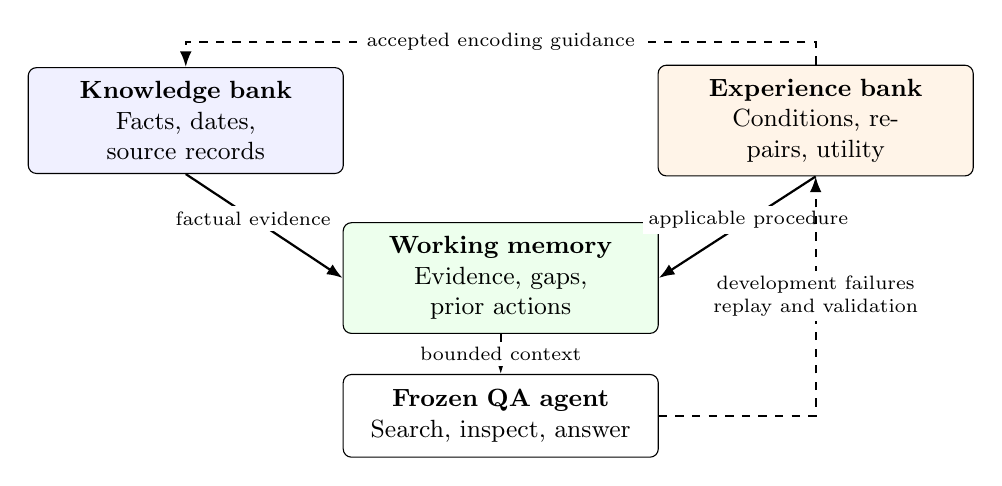
\begin{tikzpicture}[
  box/.style={draw,rounded corners=3pt,align=center,font=\small,
    minimum height=1.05cm,text width=3.65cm,inner sep=5pt},
  arrow/.style={-{Latex[length=2mm]},thick},
  lab/.style={font=\scriptsize,align=center,fill=white,inner sep=2pt}]
\node[box,fill=blue!6] (k) at (0,0) {\textbf{Knowledge bank}\\Facts, dates, source records};
\node[box,fill=orange!9] (e) at (8.0,0) {\textbf{Experience bank}\\Conditions, repairs, utility};
\node[box,fill=green!7] (w) at (4.0,-2.0) {\textbf{Working memory}\\Evidence, gaps, prior actions};
\node[box,text width=3.65cm] (a) at (4.0,-3.75) {\textbf{Frozen QA agent}\\Search, inspect, answer};
\draw[arrow] (k.south) -- node[lab,pos=.43]{factual evidence} (w.west);
\draw[arrow] (e.south) -- node[lab,pos=.43]{applicable procedure} (w.east);
\draw[arrow] (w.south) -- node[lab]{bounded context} (a.north);
\draw[arrow,dashed] (a.east) -- (8.0,-3.75) -- node[lab,pos=.5]{development failures\\replay and validation} (e.south);
\draw[arrow,dashed] (e.north) -- (8.0,1.0) -- node[lab]{accepted encoding guidance} (0,1.0) -- (k.north);
\end{tikzpicture}
\caption{Two persistent banks and one transient state. Solid arrows are used
while answering; dashed arrows describe development-time improvement and its
effect on future memory construction. Source records are part of the knowledge
bank, not an additional learned memory.}
\label{fig:framework}
\end{figure}

\subsection{Knowledge: Preserve Claims and Their Sources}
A knowledge record contains a claim, its participants, temporal scope, source
turn identifiers, and a version. The same bank retains the original source
records for bounded inspection or re-encoding. A writer processes history in
chronological batches without access to future questions or gold answers.
It preserves dated changes instead of replacing every old claim with the latest
one. A correction links the revised claim to the affected version; incompatible
claims remain explicit until their scopes can be resolved.

The default index combines dense and lexical retrieval. Accepted encoding
procedures may change the writer's extraction instructions, such as preserving
the time of a state change or retaining both participants in a relation.
These procedures are selected from properties of the incoming batch, not from
an unseen evaluation question. At query time, a bounded source inspection may
recover an omitted distinction. Such access is logged and charged to the
retrieval and context budgets.

\subsection{Experience: Store Conditional Repair Procedures}
An experience entry has the form
\begin{equation}
    e=(c,z,p,u),\qquad z\in\{\text{encode},\text{retrieve},\text{answer}\},
\end{equation}
where $c$ specifies its applicability, $z$ names the operation to change,
$p$ is a short procedure, and $u$ records validation support and subsequent
successes or failures. For example, a procedure may require searching adjacent
dated sessions when a question asks about a change of state. It must not store
a benchmark answer as the procedure. Names, answer strings, and conversation
identifiers are removed from reusable guidance; development source identifiers
remain in an audit record that is not exposed as answer context.

Applicability is filtered by operation and observable problem features before
semantic ranking. Retrieval returns at most two procedures. A validated
procedure has priority over an untested candidate, and a contradicted or
repeatedly unhelpful entry is retired. This bank transfers problem-solving
experience across conversations, while the knowledge bank supplies the facts
for the current conversation.

\subsection{Working State: Track Evidence and Unresolved Needs}
Working memory is a compact record of the question, evidence identifiers,
unresolved entities or dates, conflicts, attempted operations, and remaining
budget. It is initialized for each question and discarded afterward. The agent
does not persist a free-form reasoning transcript as factual memory.

At step $t$, the controller retrieves applicable experience and updates the
working state from the actual retrieval or inspection result:
\begin{equation}
\begin{split}
 P_t &= \operatorname{RetrieveExperience}(\EB_n,q_i,\WM_{i,t}),\\
 (R_t,a_t) &= \operatorname{Act}(\Model,q_i,\WM_{i,t},P_t,\KB_i),\\
 \WM_{i,t+1} &= \operatorname{Update}(\WM_{i,t},R_t,a_t).
\end{split}
\end{equation}
Available actions are knowledge search, source inspection, comparison of
retrieved evidence, and answer or abstain. A missing fact is marked resolved
only when a returned source supports it. The agent stops when the evidence is
sufficient or the action budget is exhausted. Experience may guide the search
or interpretation, but cannot itself serve as factual evidence.

\section{Learning from Failure}
\label{sec:learning}
The experience bank starts empty. Development runs log the knowledge version, retrieved records, working
states, actions, cited sources, answer, and feedback. Gold answers and evidence
annotations may supervise this development process; they are unavailable during
held-out inference. A failure opens a small, predefined repair space:

\begin{center}
\small
\begin{tabularx}{\linewidth}{@{}p{2.0cm}XX@{}}
\toprule
Repair target & Diagnostic evidence & Candidate intervention \\
\midrule
Encoding & Relevant source exists, but its claim or scope is missing from the bank & Re-encode a bounded source region with revised extraction guidance \\
Retrieval & Supporting records exist but were absent from the answer context & Change query decomposition, entity expansion, or temporal filtering \\
Answering & Supporting evidence reached the reader but was misused & Require evidence comparison, date resolution, or calibrated abstention \\
\bottomrule
\end{tabularx}
\end{center}

The learner proposes one local procedure for each implicated target and replays
the failed development examples with the model, sources, and resource limits
held fixed. A probe changes one operation at a time. Its outcome indicates a
useful intervention, not a uniquely identified causal explanation; ambiguous
failures may remain unresolved. An encoding repair must produce source-backed
records, and an answering repair cannot inject the gold answer into the prompt.

Let $F$ be the failed development batch and $V$ a separate validation set. A
candidate procedure $p$ is admitted only when it improves mean QA score on $F$,
does not reduce mean QA score on $V$, and respects the resource limits:
\begin{equation}
\operatorname{Accept}(p)=
\mathbf{1}\{\Delta_F(p)>0\;\land\;\Delta_V(p)\geq0\;\land\;C(p)\leq B\}.
\end{equation}
Replays use matched seeds and starting knowledge snapshots. A failed candidate
does not alter deployed experience. The writer is versioned with the accepted
encoding procedures so that future banks can be rebuilt from their histories.
Within a frozen evaluation run, source inspection changes only the current
working context; answering one question cannot improve the bank for the next.

The loop is bounded to three development rounds and a bank of at most 64
procedures. It retains generalized guidance rather than an ever-growing set of
answer examples. The learner receives validation acceptance decisions, while
test histories, questions, labels, and scores never enter procedure generation
or selection. This is continual adaptation through external memory; no model
parameters are optimized.

\section{Experimental Protocol}
\label{sec:experiments}
\textbf{Empirical status.} The experiments below are specified but not executed.
No accuracy, cost reduction, significance claim, or synthetic performance curve
is reported as an observed result.

\paragraph{Benchmarks and separation.}
We will evaluate the released LoCoMo conversational QA data
\citep{locomo} and the cleaned LongMemEval-S data \citep{longmemeval}.
LoCoMo tests single-hop, multi-hop, temporal, open-domain, and adversarial
questions; LongMemEval tests long histories, updates, temporal reasoning, and
cross-session recall. The primary protocol uses five outer folds. Each
LoCoMo fold assigns six whole conversations to experience development, two to
validation, and two to test; each conversation is tested once. LongMemEval
uses approximately 60/20/20 percent development/validation/test per fold,
grouping examples with shared user histories or answer-bearing sessions before
assignment. Every released example is evaluated only in its held-out fold.
Exact group sizes and manifests must be published. These are cross-fitted
research scores, not the official fixed-bank leaderboard setting.

Each test history is ingested from scratch using the frozen experience learned
outside its fold. Neither benchmark's test feedback updates either bank.
Chronological batches within the development partition supply the experience
stream; this ordering is an experimental schedule, not a claim that unrelated
benchmark histories form one natural user timeline.

\paragraph{Shared configuration and comparison.}
The planned primary reader and learner are Qwen3-8B, with Qwen3-Embedding-4B
for dense retrieval. Temperature is zero and paired trials use three seeds.
The primary per-step memory budget is 4,096 reader tokens, allocated as up to
3,072 for evidence, 512 for experience, and 512 for working state. Unused space
is available to evidence. A question permits at most three retrieval or
inspection actions; the same total memory budget and action ceiling apply to
controlled baselines. We will report the 2,048/8,192-token budgets only as a
sensitivity curve, and cap experience development at three rounds.

Comparisons include raw-history hybrid RAG, Mem0, A-MEM, SimpleMem, LightMem,
and a LangMem store manager. Every method uses the same reader and embedding
models. We will pin source commits and report any adapters or deviations from
native execution; a modified implementation will not be labeled a paper
reproduction. Full-context answering is a separate reference with its larger
input budget explicitly reported. An additional controlled EM--WM baseline
uses experience and working state with fixed knowledge encoding, inspired by
Recuris; it is an adaptation for QA, not an official Recuris result.

\subsection{Answer Quality and Cost}
The main comparison will report LoCoMo token F1 over the four answerable
categories, category-level scores, and adversarial abstention separately.
LongMemEval uses the official question-type-aware judging procedure. A pinned
GPT-4o judge is planned, with its exact snapshot, prompt, and raw decisions
recorded; the same judge is used across systems. Evidence recall is reported
from source turns for LoCoMo and supporting sessions for LongMemEval, with
abstention cases excluded from evidence recall. These units are not pooled.
An experience entry never counts as retrieved factual support.

One main results table will pair answer quality with retrieved tokens, median
and tail latency, and total model calls. Construction, development replay,
and query-time costs will be shown separately, alongside amortized cost per
answered question. Paired uncertainty estimates will resample entire
conversations or shared-history groups, rather than treating correlated
questions as independent.

\subsection{Contribution of the Three Memories}
A single controlled ablation table will compare the full framework with:
knowledge only; knowledge plus experience without an explicit working state;
knowledge plus working state with no learned experience; and one pooled store
containing the same knowledge and procedure records. All variants keep the same
source archive, action ceiling, reader, and total token budget; removed memory
allocations return to factual evidence. A fixed, length-matched set of
human-written procedures tests whether learned experience helps beyond generic
advice. We will also disable encoding repair while keeping the rest of the
loop intact to isolate improvement of factual storage from query-time control.
Failure cases will be inspected through the logged availability, retrieval,
and use of the annotated evidence.

\subsection{Continual Transfer and Memory Growth}
We will evaluate frozen experience snapshots after each development round on
untouched test folds without selecting a snapshot by test score. A single curve
will show answer quality against accumulated experience and total development
cost; a companion retention measure will track previously solved validation
questions. A cross-benchmark test will learn experience on LoCoMo and apply it
to LongMemEval, and reverse the direction, rebuilding all target knowledge
banks from their own histories without target feedback. This separates
procedural transfer from memorizing a benchmark's answers. Source-side
validation fixes all settings before the transfer run.

\section{Related Work and Scope}
Fact-oriented systems extract, connect, and consolidate information for later
recall, including Mem0, A-MEM, SimpleMem, and LightMem
\citep{mem0,amem,simplemem,lightmem}. Our knowledge bank adopts this setting;
the proposed addition is learning conditional interventions from its failures.
Reflexion, AdaMEM, and ReMe reuse feedback or execution experience
\citep{reflexion,adamem,reme}. LangMem exposes semantic, episodic, and procedural
memory as configurable primitives \citep{langmem}.

Recuris is the closest control-level comparison: it couples experience with
verified working state and updates skills, state specifications, invocation
policies, and checkers from failed traces \citep{recuris}. We do not claim
these general principles as new. Our specific target is factual omission and
evidence access in a separately scoped conversational knowledge bank. The
encoding-repair ablation and the fixed-encoding EM--WM control are necessary
to determine whether that distinction has measurable value.

\section{Limitations and Conclusion}
The design depends on the fidelity of source attribution and development
feedback. Replay can identify a helpful repair without proving the true cause
of failure. Repeated validation may overfit a small development set, and
LoCoMo has few independent conversations. Keeping source records increases
storage cost; learned procedures may also transfer poorly across domains.
These limitations must be evaluated rather than assumed away.

The framework separates factual support, reusable experience, and current
evidence state. Its central hypothesis is that experience should change how
knowledge is retained and accessed, while remaining distinct from the facts
used to answer. LoCoMo and LongMemEval provide a focused test of that
hypothesis. Until those experiments are completed, effectiveness remains an
open empirical question.

\subsection*{AI Use Statement}
Generative AI assisted the development of the proposed architecture, literature
comparison, experimental protocol, prose, and LaTeX for this working draft.
No framework implementation, benchmark runs, or empirical results were
generated for this manuscript. Human authors must review the method,
references, and final disclosure before submission.

\clearpage
\bibliography{references}
\bibliographystyle{iclr2027_conference}
\end{document}
